\documentclass[11pt,a4paper]{article}

\usepackage[utf8]{inputenc}
\usepackage[T1]{fontenc}
\usepackage[english]{babel}
\usepackage{amsmath}
\usepackage{booktabs}
\usepackage{graphicx}
\usepackage{geometry}
\usepackage{hyperref}
\usepackage{listings}
\usepackage{xcolor}

\geometry{margin=2.8cm}
\hypersetup{colorlinks=true, linkcolor=blue, citecolor=blue, urlcolor=blue}
\lstset{basicstyle=\ttfamily\small, frame=single, breaklines=true}

\title{A Two-Dimensional Smoothed Particle Hydrodynamics Solver}
\author{Author Name}
\date{\today}

\begin{document}

\maketitle
\begin{abstract}
This paper documents the design and evaluation of a small two-dimensional smoothed
particle hydrodynamics (SPH) solver. The implementation combines particle-based
fluid dynamics, radius-based neighbor search, numerical integration, and an
interactive renderer.
\end{abstract}

\tableofcontents

\section{Introduction}

Particle-based methods are useful for simulating fluids with free surfaces and
changing topology. Smoothed particle hydrodynamics represents a continuum by a
set of moving particles and approximates field quantities using a smoothing
kernel \cite{lucy1977,morris1997}.

The goal of this project is to implement and inspect a compact two-dimensional
SPH solver in C++17. The application includes density and pressure estimation,
viscosity, gravity, boundary particles, and an interactive SFML renderer. This
paper describes the numerical model, the software architecture, and the tests
used to assess the implementation.

\section{Research Questions}

The evaluation focuses on three questions:
\begin{enumerate}
    \item Does the solver preserve the expected qualitative behavior of a small
    fluid scene?
    \item How does the radius-based neighbor search affect the simulation's
    computational work?
    \item Which implementation parameters have the greatest visible effect on
    stability and motion?
\end{enumerate}
\section{Methodology}

\subsection{SPH Approximation}

For a quantity $A$ evaluated at particle $i$, the SPH approximation is written
as
\begin{equation}
    A_i \approx \sum_j m_j \frac{A_j}{\rho_j} W(\lVert \mathbf{r}_i-\mathbf{r}_j\rVert,h),
\end{equation}
where $m_j$ is the particle mass, $\rho_j$ is the density, $h$ is the smoothing
length, and $W$ is a compact-support kernel \cite{lucy1977,monaghan1992}.
We use the two-dimensional cubic spline with support radius $2h$,
\begin{equation}
    W(q,h) = \frac{5}{14\pi h^2}
    \begin{cases}
        (2-q)^3 - 4(1-q)^3, & 0 \le q < 1,\\
        (2-q)^3,            & 1 \le q < 2,\\
        0,                  & q \ge 2,
    \end{cases}
    \qquad q = \frac{\lVert \mathbf{r}_i-\mathbf{r}_j\rVert}{h}.
\end{equation}

Particles are initialised on a square lattice with spacing $\Delta x$ and
carry the mass $m = \rho_0 \Delta x^2$, so that a particle inside a regular
lattice sums to the rest density $\rho_0$. The smoothing length is set to
$h = 1.3\,\Delta x$, which gives about 20 neighbours per particle. Larger ratios
make the cubic spline prone to the pairing instability \cite{dehnen2012}, in
which particles clump into rows; this is examined in
Section~\ref{sec:pairing}.

\subsection{Density and Equation of State}

The density is obtained by direct summation over all particles within the
kernel support, including the particle itself and the wall particles,
\begin{equation}
    \rho_i = m_i W(0,h) + \sum_{j \ne i} m_j W_{ij}.
\end{equation}
The fluid is treated as weakly compressible \cite{monaghan1994,becker2007}.
Pressure follows the Tait equation
\begin{equation}
    p_i = B\left[\left(\frac{\rho_i}{\rho_0}\right)^{\gamma} - 1\right],
    \qquad B = \frac{\rho_0 c^2}{\gamma}, \qquad \gamma = 7,
    \label{eq:tait}
\end{equation}
where $c$ is the numerical speed of sound; negative pressures are set to zero
to avoid tensile clumping at the free surface. The density error scales with
the squared Mach number $\mathrm{Ma}^2 = (v/c)^2$, so $c$ is chosen as ten times
the largest expected flow speed. Estimating that speed by free fall from the top
of the fluid body of height $H$ gives
\begin{equation}
    c = 10\sqrt{2gH},
\end{equation}
which targets density errors of about one percent.

\subsection{Momentum Equation}

The acceleration of a fluid particle is the sum of a pressure term, a viscous
term and gravity,
\begin{align}
    \mathbf{a}_i^{p} &= -\sum_j m_j \left(\frac{p_i}{\rho_i^2} + \frac{p_j}{\rho_j^2}\right) \nabla_i W_{ij},\\
    \mathbf{a}_i^{\nu} &= 2\nu \sum_j \frac{m_j}{\rho_j}
        \frac{\mathbf{v}_{ij}\cdot\mathbf{r}_{ij}}{\lVert\mathbf{r}_{ij}\rVert^2 + 0.01h^2}\,\nabla_i W_{ij},\\
    \mathbf{a}_i &= \mathbf{a}_i^{p} + \mathbf{a}_i^{\nu} + \mathbf{g},
\end{align}
with $\mathbf{r}_{ij} = \mathbf{r}_i - \mathbf{r}_j$ and
$\mathbf{v}_{ij} = \mathbf{v}_i - \mathbf{v}_j$. The symmetric pressure term
conserves linear momentum; the viscous term follows
\cite{monaghan1992,morris1997} and also damps the acoustic oscillations that a
weakly compressible fluid carries.

\subsection{Boundary Conditions}

Walls are built from fixed particles placed on the same lattice as the fluid.
Enough layers are used to fill the full kernel support of a fluid particle
touching the wall ($\lceil 2h/\Delta x \rceil = 3$ layers for $h = 1.3\Delta x$),
so that wall particles enter the density sum like fluid at rest density.

Wall particles carry no state of their own, so a pressure has to be assigned to
them. If the wall term used only $p_i/\rho_i^2$ \cite{akinci2012}, the wall
would provide half the support that a fluid neighbour provides; the first fluid
layer then has to compress until its pressure is roughly doubled, which pushes
the second layer away and leaves a visible gap above the floor. Instead the wall
pressure is extrapolated from the surrounding fluid following
Adami et al.~\cite{adami2012},
\begin{equation}
    p_b = \frac{\sum_f p_f W_{bf} + \mathbf{g}\cdot\sum_f \rho_f\,(\mathbf{r}_b - \mathbf{r}_f)\,W_{bf}}{\sum_f W_{bf}},
\end{equation}
where the sums run over the fluid neighbours $f$ of the wall particle $b$ and the
second term adds the hydrostatic pressure difference across the wall. The wall
density $\rho_b$ follows from inverting Eq.~\eqref{eq:tait}, and the fluid--wall
pressure force uses the same symmetric form as the fluid--fluid force.

As a safety net against penetration during violent impacts, a fluid particle
that comes closer than $\Delta x/2$ to a wall particle is projected back to that
distance and its normal velocity is reflected with a restitution of $0.5$.
Fluid at rest sits a full spacing away from the wall, so the projection does not
act in quiescent regions.

\subsection{Time Integration}

Positions and velocities are advanced with the semi-implicit (symplectic) Euler
scheme,
$\mathbf{v}^{n+1} = \mathbf{v}^{n} + \Delta t\,\mathbf{a}^{n}$,
$\mathbf{r}^{n+1} = \mathbf{r}^{n} + \Delta t\,\mathbf{v}^{n+1}$.
The time step is chosen adaptively in every substep as the most restrictive of
the acoustic CFL, force, and viscous conditions \cite{monaghan1992},
\begin{equation}
    \Delta t = \min\left(
        0.4\,\frac{h}{c + \max_i \lVert\mathbf{v}_i\rVert},\;
        0.25\sqrt{\frac{h}{\max_i \lVert\mathbf{a}_i\rVert}},\;
        0.125\,\frac{h^2}{\nu}
    \right).
\end{equation}
Each rendered frame advances the simulation by $1/60\,\mathrm{s}$, split into as
many substeps as these limits require. For the stiff fluids used here the
acoustic condition dominates.

\subsection{Neighbour Search}

Neighbour lists are rebuilt once per substep by testing all particle pairs
against the kernel support radius $2h$. The cost of this search is
$\mathcal{O}(N^2)$; it is adequate for the scene sizes used in this work
(about $1.6\times10^3$ particles) but is the main limitation for larger scenes.

\subsection{Software Structure}

The solver is separated into the following components:
\begin{itemize}
    \item \texttt{Particle} stores particle state and physical properties.
    \item \texttt{NeighborSearch} constructs local particle neighborhoods.
    \item \texttt{SPHSolver} performs the density, wall-pressure, force, and
          integration steps and chooses the adaptive time step.
    \item \texttt{Scenes} builds the test scenes (tank walls, fluid body, and
          matching solver parameters).
    \item \texttt{Renderer} displays the scene and exposes runtime controls.
\end{itemize}

This separation allows the numerical code to be tested and run without an
interactive graphics window. A headless program (\texttt{sph\_experiments})
runs all experiments of Section~\ref{sec:results} and writes their data as CSV
files, from which the figures are generated.

\subsection{Experimental Setup}

All quantities are given in screen units (pixels and seconds). Results are
reported in dimensionless form ($p/\rho_0 g H$, $Z/a$, $T = t\sqrt{g/a}$), so the
choice of units does not affect them. Two scenes are used
(Table~\ref{tab:setup}):
\begin{itemize}
    \item \textbf{Hydrostatic column.} An open tank of width $300\,\mathrm{px}$ is
          filled to $H = 400\,\mathrm{px}$ with fluid at rest. The column has to
          settle to the hydrostatic pressure $p = \rho_0 g d$ at depth $d$.
    \item \textbf{Dam break.} A fluid column of width $a = 200\,\mathrm{px}$ and
          height $H = 400\,\mathrm{px}$ (aspect ratio $n^2 = H/a = 2$) stands in
          the lower-left corner of a closed tank of width $800\,\mathrm{px}$ and
          collapses under gravity at $t = 0$ \cite{martin1952}.
\end{itemize}

\begin{table}[ht]
    \centering
    \caption{Default parameters of both scenes. Parameter studies vary one
    quantity at a time.}
    \label{tab:setup}
    \begin{tabular}{lll}
        \toprule
        Quantity & Symbol & Value \\
        \midrule
        Particle spacing & $\Delta x$ & $10\,\mathrm{px}$ \\
        Smoothing length & $h$ & $13\,\mathrm{px}$ ($1.3\,\Delta x$) \\
        Rest density & $\rho_0$ & $300$ \\
        Gravity & $g$ & $200\,\mathrm{px/s^2}$ \\
        Speed of sound & $c$ & $10\sqrt{2gH} = 4000\,\mathrm{px/s}$ \\
        Viscosity & $\nu$ & $150\,\mathrm{px^2/s}$ \\
        Fluid / wall particles (column) & & $1200$ / $420$ \\
        Fluid / wall particles (dam break) & & $800$ / $828$ \\
        Frame time & & $1/60\,\mathrm{s}$ \\
        \bottomrule
    \end{tabular}
\end{table}

\section{Results}
\label{sec:results}

All data in this section are produced by the experiment runner
\texttt{sph\_experiments} and plotted by the script
\texttt{plots/make\_plots.py}; rerunning both regenerates every figure.

\subsection{Correctness Tests}

The repository includes CTest unit tests for the neighbour search, for the
density summation (an isolated particle carries $m\,W(0,h)$; a particle inside a
regular lattice recovers $\rho_0$ to within $0.01\,\%$), for the slope of the
equation of state ($\partial p/\partial\rho = c^2$ at $\rho_0$), and a short
hydrostatic-column regression test that checks the CFL limit, containment, the
density error and the hydrostatic pressure profile.

\subsection{Hydrostatic Column}

Figure~\ref{fig:hydro-pressure} compares the particle pressures of the settled
column with the hydrostatic solution $p = \rho_0 g d$. Instantaneous pressures
scatter around the solution with a mean deviation of about $10\,\%$ of
$\rho_0 g H$. Averaged over $2\,\mathrm{s}$, the scatter shrinks to $2.4\,\%$
and the mean pressure below the surface layer matches the hydrostatic value to
within $0.3\,\%$. The instantaneous scatter is therefore not a bias but acoustic
noise: pressure waves travel through the column much faster than the frame
rate.

\begin{figure}[ht]
    \centering
    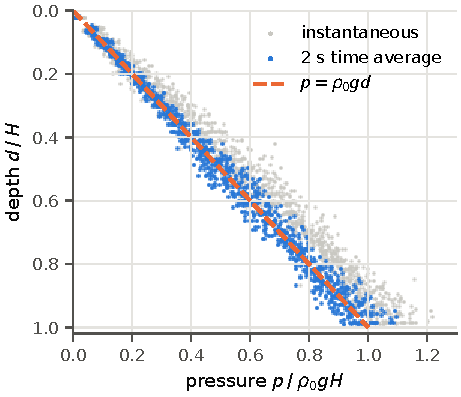
\includegraphics{figures/hydro_pressure.pdf}
    \caption{Pressure against depth in the settled hydrostatic column
    ($t = 8$--$10\,\mathrm{s}$). Grey: instantaneous particle pressures; blue:
    pressures averaged over $2\,\mathrm{s}$; dashed: hydrostatic solution.}
    \label{fig:hydro-pressure}
\end{figure}

Figure~\ref{fig:hydro-settling} shows how the column settles. The particles
start on a lattice at exactly $\rho_0$ and therefore without pressure, so the
column first falls slightly and then oscillates acoustically. Viscosity damps
the mean kinetic energy by more than an order of magnitude within
$10\,\mathrm{s}$. The maximum density error settles at $0.56\,\%$ (mean
$0.25\,\%$), close to the estimate $\Delta\rho/\rho_0 \approx gH/c^2 = 0.5\,\%$
for the compression at the bottom of the column. The adaptive time step settles
at $\Delta t \approx 1.2\times10^{-3}\,\mathrm{s}$, i.e.\ 13 substeps per frame.

\begin{figure}[ht]
    \centering
    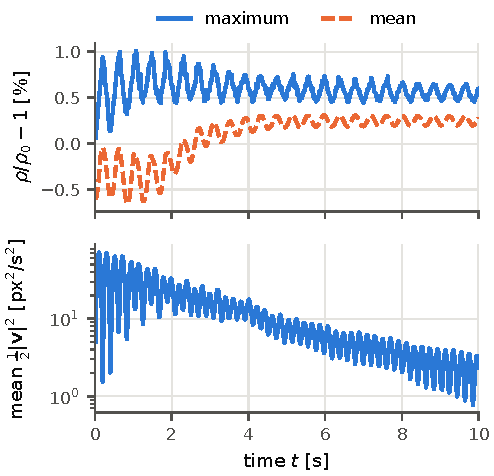
\includegraphics{figures/hydro_settling.pdf}
    \caption{Settling of the hydrostatic column: density error (top) and mean
    kinetic energy per unit mass (bottom, logarithmic).}
    \label{fig:hydro-settling}
\end{figure}

\subsection{Dam Break}

Figure~\ref{fig:dam-snapshots} shows the collapse of the water column, coloured
by pressure. The front position $Z$ along the floor is shown in
Fig.~\ref{fig:dam-front} in the dimensionless form of Martin and
Moyce~\cite{martin1952}. The front reaches $Z/a = 1.87$ at $T = 1$ and
$3.62$ at $T = 2$, and hits the opposite wall ($Z/a = 4$) at $T = 2.18$. After
an initial acceleration phase the front moves at a nearly constant speed. The
shallow-water solution of Ritter~\cite{ritter1892}, $Z/a = 1 + 2nT$, assumes
that the front starts at full speed and bounds the motion from above.
% TODO: add the Martin & Moyce comparison once Latex/data/martin_moyce_n2.csv is
% filled in; SPH fronts are commonly reported to run ahead of the experiment.

\begin{figure}[ht]
    \centering
    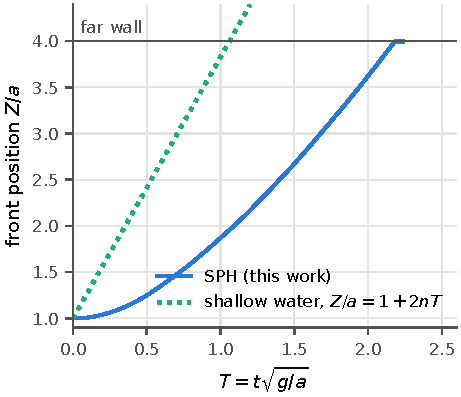
\includegraphics{figures/dam_front.pdf}
    \caption{Front position of the dam break in dimensionless form
    ($a$: initial column width, $n^2 = H/a = 2$).}
    \label{fig:dam-front}
\end{figure}

\begin{figure}[ht]
    \centering
    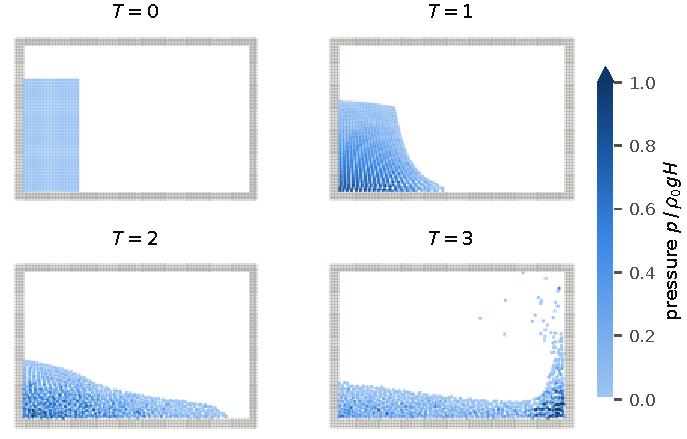
\includegraphics{figures/dam_snapshots.pdf}
    \caption{Dam break at $T = t\sqrt{g/a} = 0, 1, 2, 3$. Fluid particles are
    coloured by pressure, smoothed over $0.05\,\mathrm{s}$ per particle to
    suppress acoustic noise; wall particles are grey.}
    \label{fig:dam-snapshots}
\end{figure}

Until the impact on the right wall the maximum density error stays below
$1.5\,\%$ and the Mach number below $0.11$, as intended by the choice of $c$. At
the impact the flow is deflected upwards and the splash reaches
$\mathrm{Ma} = 0.23$, more than twice the free-fall estimate; the density error
peaks at $8.9\,\%$ for a few frames. The speed of sound chosen from a free-fall
estimate is therefore adequate for the collapse itself but marginal for the
impact.

\subsection{Speed of Sound}

The speed of sound trades compressibility against cost
(Fig.~\ref{fig:sweep-c}). Doubling $c$ reduces the density error of the
hydrostatic column roughly fourfold ($10.2\,\%$, $3.0\,\%$, $0.75\,\%$ and
$0.35\,\%$ for $c/\sqrt{2gH} = 2.5, 5, 10, 20$), following the $gH/c^2$ estimate
until noise dominates at the stiffest setting. In the dam break, the time-averaged peak density error
decreases only proportionally to $1/c$ ($8.1\,\%$ to $0.8\,\%$), because it is
set by local dynamic compression rather than by the hydrostatic load. The
number of substeps grows almost in proportion to $c$ (from 5 to 28 per frame
for an eightfold increase) since the acoustic CFL condition dominates. A stiffer fluid is also noisier: the
frame-to-frame pressure change grows from $2.3\,\%$ to $40\,\%$ of $\rho_0 g H$,
because the same small density fluctuation is multiplied by $B \propto c^2$.
The front position is insensitive to $c$ ($Z/a$ at $T = 1.5$ varies by less than
$1\,\%$).

\begin{figure}[ht]
    \centering
    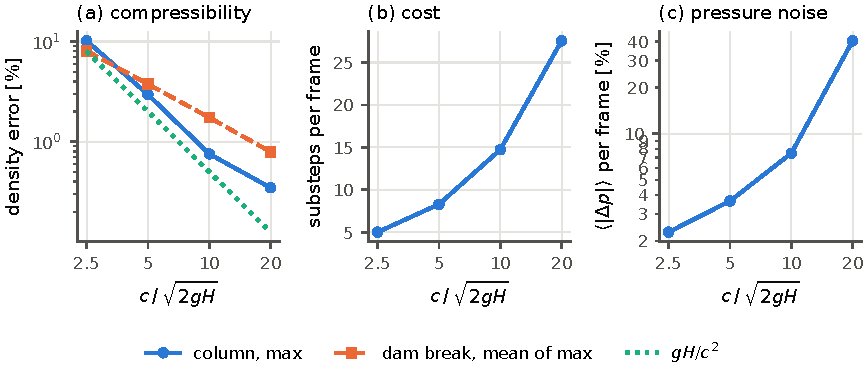
\includegraphics{figures/sweep_speed_of_sound.pdf}
    \caption{Influence of the speed of sound: (a) density error with the
    hydrostatic estimate $gH/c^2$, (b) substeps per $1/60\,\mathrm{s}$ frame
    in the dam break, (c) mean frame-to-frame pressure change in the settled
    column.}
    \label{fig:sweep-c}
\end{figure}

\subsection{Viscosity}

Viscosity mainly controls the acoustic noise (Fig.~\ref{fig:sweep-visc}). With
$\nu = 50$ the instantaneous pressure of the settled column deviates by $51\,\%$
from the hydrostatic value on average; $\nu = 150$ reduces this to $10\,\%$.
Larger viscosities do not reduce the instantaneous error further ($15$--$17\,\%$),
while the time-averaged error stays between $1.5$ and $3.2\,\%$ for all values.
The flow itself becomes slower with increasing viscosity: at $T = 1.5$ the front
has reached $Z/a = 2.74$ for $\nu = 50$ and $2.53$ for $\nu = 1000$. The default
$\nu = 150$ is a compromise between noise and numerical dissipation.

\begin{figure}[ht]
    \centering
    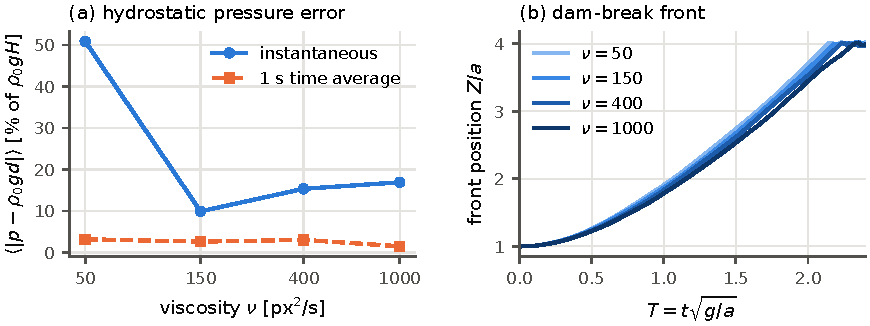
\includegraphics{figures/sweep_viscosity.pdf}
    \caption{Influence of the viscosity $\nu$: (a) mean pressure error of the
    settled column, instantaneous and averaged over $1\,\mathrm{s}$; (b) front
    position of the dam break.}
    \label{fig:sweep-visc}
\end{figure}

\subsection{Kernel Support and Pairing Instability}
\label{sec:pairing}

Figure~\ref{fig:pairing} shows how the ratio $h/\Delta x$ changes the particle
arrangement in the settled column. At $h/\Delta x = 1.2$ the particles remain
on the initial lattice, visible as sharp peaks every $10\,\mathrm{px}$; the
fluid behaves like a crystal. At $1.3$ the particles rearrange into a
disordered, liquid-like state. At $1.6$ and $2.0$ (33 and 50 neighbours instead of
about 20) the particles collapse into horizontal rows $18$--$20\,\mathrm{px}$
apart, roughly twice the initial spacing, while the spacing within a row shrinks:
the pairing instability of the cubic spline \cite{dehnen2012}. The rows also
make the pressure noisier: at $h/\Delta x = 2.0$ the frame-to-frame pressure
change is four times larger than at $1.3$. The front position of the dam break
is not affected by the ratio.

\begin{figure}[ht]
    \centering
    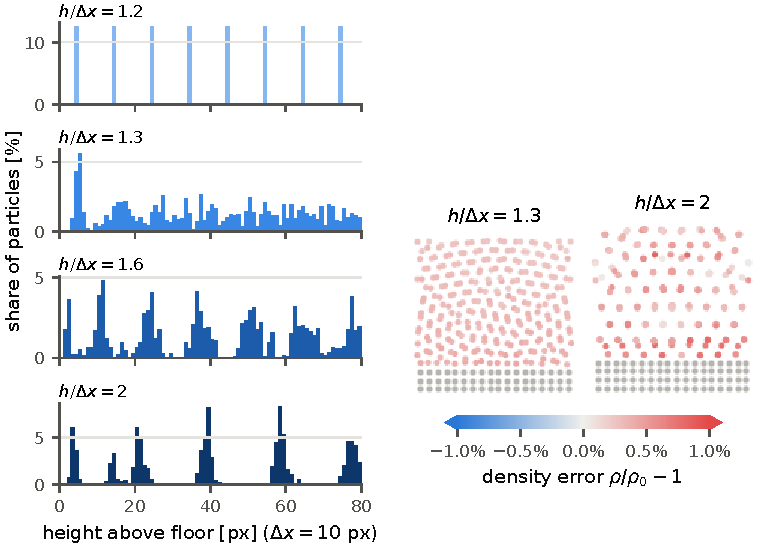
\includegraphics{figures/pairing.pdf}
    \caption{Particle arrangement in the settled hydrostatic column for
    different $h/\Delta x$. Left: distribution of particle heights above the
    floor (1\,px bins, central region). Right: the bottom of the column for
    $h/\Delta x = 1.3$ and $2.0$, coloured by density error.}
    \label{fig:pairing}
\end{figure}

\subsection{Density Fields}

Figure~\ref{fig:density-grid} compares the density error of the dam break at
$T = 2$ for all parameter variations. With $c = 2.5\sqrt{2gH}$ the lower part of
the fluid is compressed by several percent; from $c = 10\sqrt{2gH}$ on, the bulk
is within about $\pm1\,\%$ of $\rho_0$. In all runs the free surface shows a
density deficit, because the kernel support of surface particles is only
partially filled. Viscosity and $h/\Delta x$ hardly change the density field
at this resolution.

\begin{figure}[ht]
    \centering
    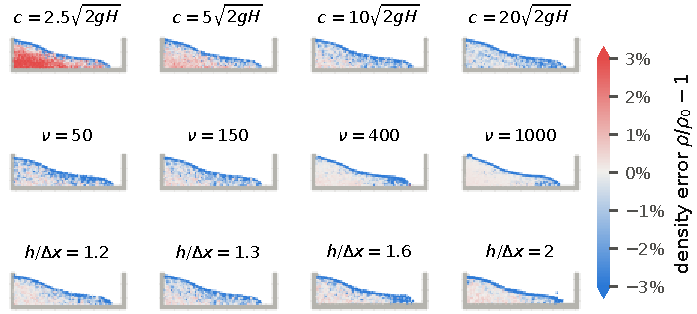
\includegraphics{figures/density_grid.pdf}
    \caption{Density error $\rho/\rho_0 - 1$ in the dam break at $T = 2$ (lower
    part of the tank). Rows vary the speed of sound, the viscosity, and the
    ratio $h/\Delta x$; the default setup is $c = 10\sqrt{2gH}$, $\nu = 150$,
    $h/\Delta x = 1.3$.}
    \label{fig:density-grid}
\end{figure}

\subsection{Discussion}

The weakly compressible model reproduces the hydrostatic pressure with a
time-averaged accuracy of a few percent and keeps density errors at about one
percent for the chosen speed of sound. Its main weakness is acoustic pressure
noise: instantaneous particle pressures scatter by about $10\,\%$ of the
hydrostatic pressure even in a fluid at rest. The interactive renderer
therefore colours particles by a per-particle moving average of the pressure.
Methods that diffuse density perturbations ($\delta$-SPH) or solve for pressure
implicitly (IISPH, DFSPH) would remove this noise at the source.

Further limitations are the $\mathcal{O}(N^2)$ neighbour search, which limits
the resolution to about $10^3$ fluid particles at interactive rates; the
projection safety net at the walls, which is not part of the SPH formulation;
and the free-fall estimate of the flow speed used to choose $c$, which
underestimates the speeds reached at the wall impact.

\section{Conclusion}

This project provides a small and inspectable SPH fluid solver with an
interactive visualization and isolated tests for its core components. The
separation between neighbor search, numerical integration, and rendering gives
the implementation a useful basis for experiments.

Future work could compare different smoothing kernels, improve boundary
handling, and benchmark spatial acceleration structures with larger particle
sets.

\bibliographystyle{plain}
\bibliography{references}

\end{document}